\chapter{腹侧前额叶皮层:基于视听内容生成目标} \label{chap:chap7}


腹侧前额叶皮层根据视觉和听觉线索生成目标,我们称之为标志,它的连接解释了为什么只有它才能做到这一点。
腹侧前额叶皮层与\textit{下颞皮层}的视觉区和\textit{上颞皮层}的听觉区以及其他前额叶皮层都有联系。
它与颞叶皮层的连接提供了视觉和听觉信号,从而建立了当前的行为环境。
眶额皮层提供了选择和结果之间的联系,有时可以在单个事件的基础上学习(第~\ref{chap:chap4}~章)。
在许多任务中,腹侧前额叶皮层根据具体物体和地点生成目标。
然而,在涉及抽象规则和策略的任务中,腹侧前额叶皮层可以生成一组或几类目标以供选择或规避。
鉴于腹侧前额叶皮层在类人猿灵长类动物中进化(第~\ref{chap:chap2}~章),我们认为它在使用视觉标志和声音信息方面具有优势,可以指导近距离和远距离的觅食选择。


\section{介绍}
\par

% As Chapter 2 points out
正如第~\ref{chap:chap2}~章所指出的,人们经常将灵长类动物描述为“视觉动物”。
原因是中央凹在早期的\textit{灵长目亚目}中进化,而三色视觉在类人猿中进化。
这些进步使这些动物及其后代能够辨别位置、颜色、形状、视觉纹理、光泽度和半透明度的微小差异。
本章回顾了类人猿使用这些视觉特征来提供觅食机会线索的证据,我们称之为标志。
正如第~\ref{chap:chap2}~章所解释的那样,我们所说的符号是指用作提示但不一定对应于整个对象的非空间景象和声音。
\par
进化已经设计出许多方法来获得觅食优势。
一些哺乳动物通过精心制作身体部位来开发资源,从而利用了它们的生态位。
大象的长鼻子使它们能够以其他哺乳动物无法做到的方式觅食。
长颈鹿的长脖子同样提供了独特的觅食机会。
我们认为,类人猿反而精心设计了某些大脑结构,包括腹侧前额叶皮层。

\begin{figure} 
	\centering
	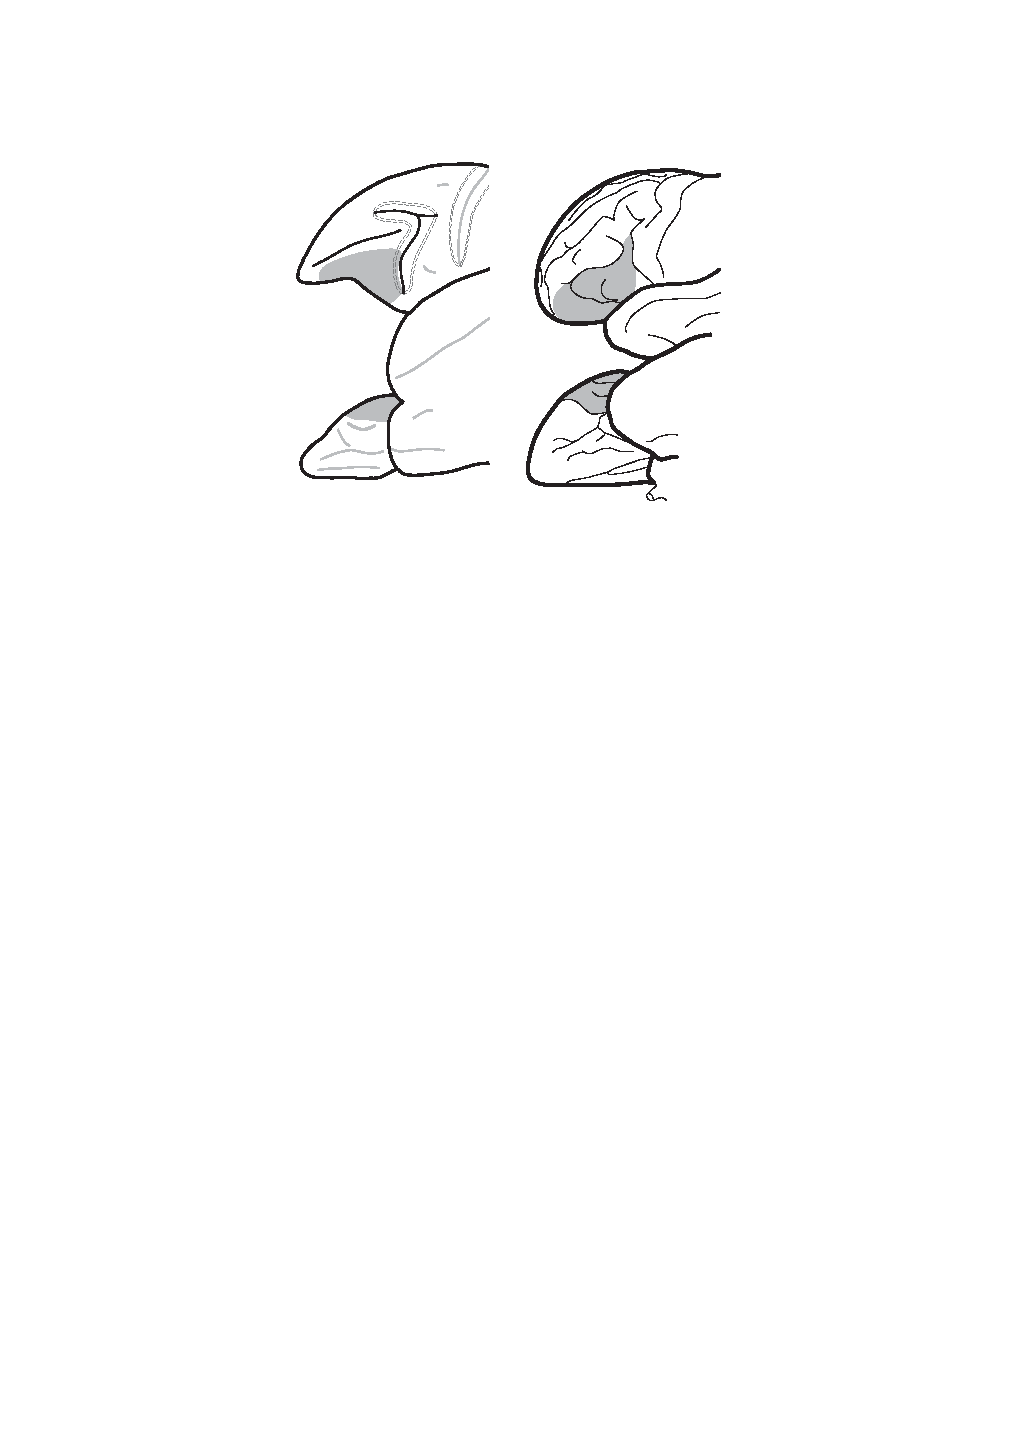
\includegraphics[width=0.7\linewidth]{chap7/7_1}
	\caption{猕猴(左)和人类(右)的腹侧前额叶皮层。
		格式如图~\ref{fig:1_2}~所示。\label{fig:7_1}}
\end{figure}
\par

前一章(第~\ref{chap:chap6}~章)解释了背侧前额叶皮层生成适合当前上下文的目标,如最近事件指定的,尤其是视觉事件。
它解释了视觉线索的顺序、位置和时间的重要性,以及其他特征,强调与后顶叶皮层的联系。
腹侧前额叶皮层与下颞叶皮层和上颞叶皮层相连。
因此,可见或可听的标志也指定了当前的上下文,类人猿可以单独使用或结合由顺序、位置和时间确定的上下文使用。



\section{区域}
\par
在猕猴中,腹侧前额叶皮层包括主沟腹侧半球的外侧凸起(图~\ref{fig:7_1})。
在人类中,同源区域位于额下回。
在两者中,腹侧前额叶皮层围绕半球的外侧末端延伸至外侧眶沟。
术语12/47由Petrides和Pandya设计,反映了他们认为人类的47区与猴子的12区同源的观点\cite{petrides2002comparative}。
\par
就细胞结构区域而言,腹侧前额叶皮层包括猕猴的45区和12/47区(见图~\ref{fig:1_2})。
在人类中,腹侧前额叶皮层包括区域45和47。


\section{连接}
\begin{figure}
	\centering
	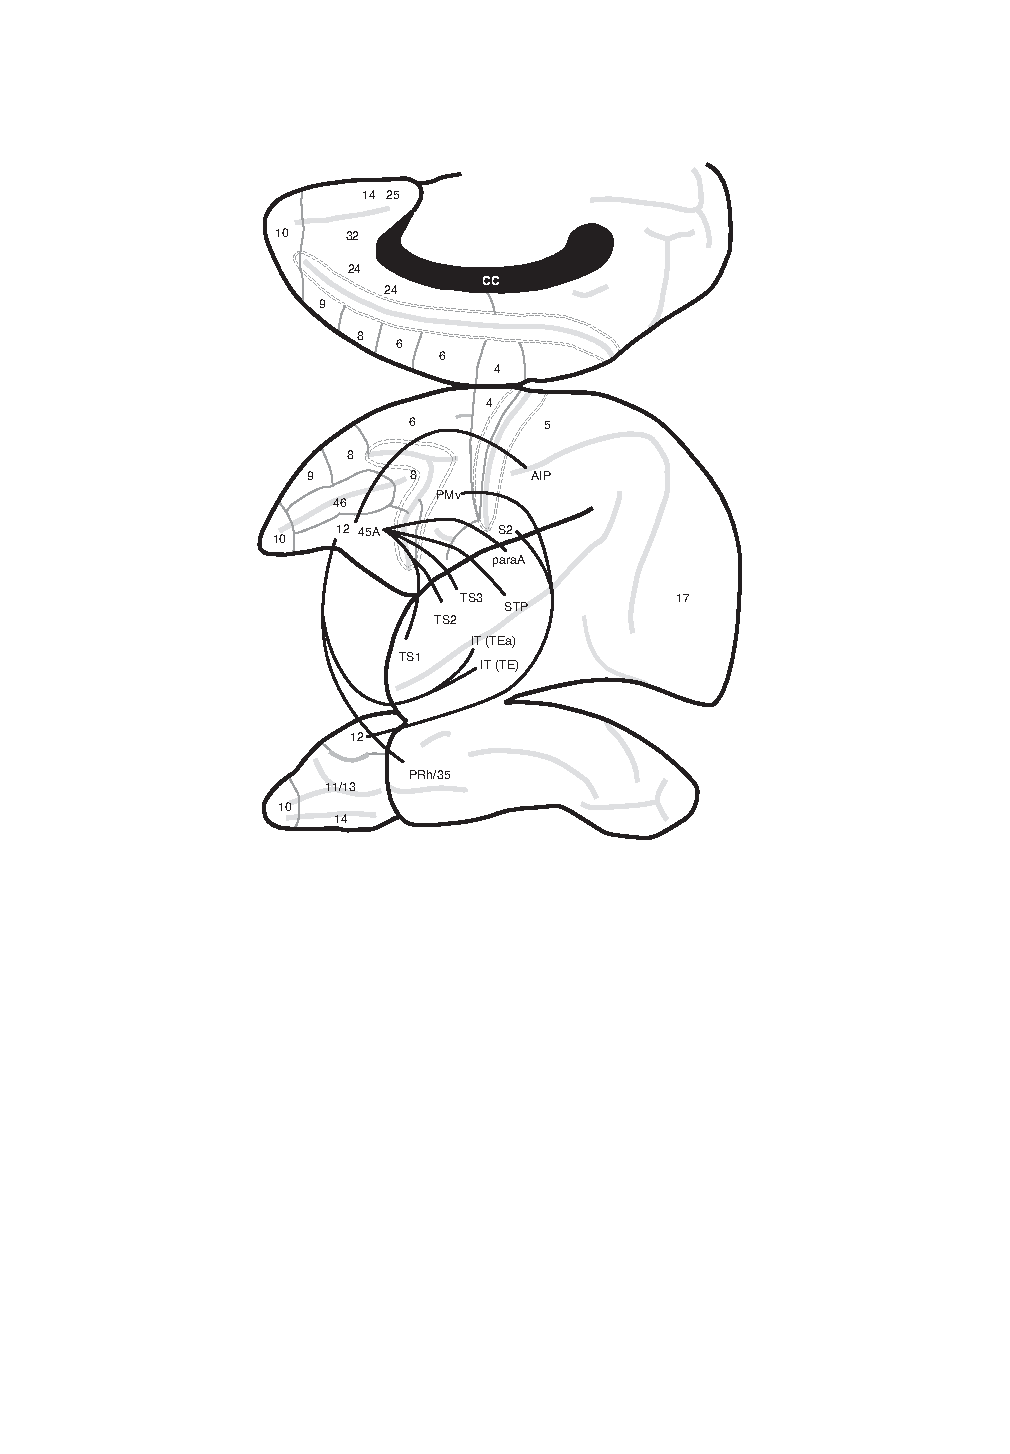
\includegraphics[width=0.7\linewidth]{chap7/7_2}
	\caption{腹侧前额叶皮层的选定连接。
		图~\ref{fig:1_4}~和图~\ref{fig:1_5}~给出了脑沟和区域的名称。
		线连接一些与腹侧前额叶皮层具有直接轴突连接的区域,除非另有说明,否则假定它们是相互的。\label{fig:7_2}}
\end{figure}


图~\ref{fig:7_2}~显示了腹侧前额叶皮层中皮层和皮层之间的连接。
有几个特点很突出:
\begin{enumerate}
\item 如前所述,腹侧前额叶皮层与颞叶紧密相连。
腹侧前额叶皮层与下颞叶皮层\cite{ungerleider1989projections,webster1994connections}和上颞叶皮层\cite{seltzer1996overlapping,petrides2002comparative}相互联系。
格式如图~\ref{fig:1_2}~所示。
它也与鼻周皮层有联系\cite{suzuki1994perirhinal,saleem2008complementary},尽管没有那么多。
\par


这些联系有两个含义。
首先,腹侧前额叶接收有关指定行为环境的信号或标志的信息。
下颞叶皮层在辨别颜色、形状和视觉纹理方面起着至关重要的作用\cite{huxlin2000perceptual}。
上颞皮层参与声音识别\cite{tian2001functional}和声音序列\cite{micheyl2005perceptual},包括其他动物的叫声\cite{rauschecker1995processing}。 
\par


其次,到达腹侧前额叶皮层的信息来自高级和中级视觉区域,而不是来自低级视觉区域。
通过高阶视觉,我们指的是一个物体特征的广泛结合,这是鼻周皮层所代表的\cite{murray2007visual}。
相比之下,下颞区,如TE区,构建了介于整个对象的表示及其基本特征之间的中级连词\cite{murray2007visual}。
最尾侧的视觉区域构建低阶连词,一些代表基本特征,但这些区域不投射到腹侧前额叶皮层\cite{webster1994connections}。
在这方面,腹侧前额叶皮层的连接与尾侧前额叶皮层的连接不同(第\ref{chap:chap5}章)。

\item 腹侧前额叶皮层还与次级体感皮层附近的一组复杂区域相互连接\cite{petrides2002comparative}。
因此,腹侧前额叶皮层接收来自视觉、听觉和躯体感觉皮层的多模式输入。
次级体感皮层内部和周围的皮层有助于物体的触觉辨别\cite{mishkin1979analogous},而鼻周皮层对于通过视觉或触觉识别物体至关重要\cite{goulet2001neural,murray2007visual}。

\item 腹侧前额叶皮层接收来自下顶叶区PG的输入\cite{petrides2002comparative}。
此连接可能会提供有关对象位置的信息。
腹侧前额叶皮层还接收来自后顶叶区域\textit{前顶叶}的输入,这似乎在猴子拾起物体时使用视觉来校准抓握方面发挥作用\cite{fogassi2001cortical}。

\item 腹侧前额叶皮层(区域 12/47)与腹侧前运动皮层的延髓部分有很强的联系。 
最近的一份报告称这部分运动前皮层区域为 F5a\cite{gerbella2011cortical},第~\ref{chap:chap2}~章提到该区域似乎控制手和嘴的运动。 

\item 腹侧前额叶皮层也与杏仁核有关。
一些神经解剖学家将这些描述为广泛的\cite{amaral1984amygdalo,stefanacci2002some},但其他人则认为它们是稀疏的\cite{carmichael1995limbic,price2010neurocircuitry}。
无论如何,与杏仁核的连接可能会提供更新的估值,如第~\ref{chap:chap3}~章和第~\ref{chap:chap4}~章所解释的那样,直接连接到腹侧前额叶皮层或通过眶额皮层间接连接。
包括下颞叶皮层\cite{horel1975partial}或杏仁核\cite{horel1975partial}在内的损伤会影响物体看起来有吸引力还是令人厌恶,并且两者都与腹侧前额叶皮层有关。
\end{enumerate}



\subsection{总结}
腹侧前额叶皮层从下颞叶皮层和上颞叶皮层接收有关视觉和听觉信号的信息,并且它可以将当前行为背景的这些方面与来自杏仁核或眶额皮层的结果信息整合\cite{barbas1989architecture},或两者皆有。


\section{视觉和听觉条件任务}
\par
鉴于其与颞叶的联系,腹侧前额叶皮层可以使用有关视觉和听觉环境的信息来生成目标。 
实验室实验可以通过使用条件任务来测试这种能力。 
这些任务涉及视觉和听觉条件任务 199 上下文和适当目标之间的任意映射。
因此,例如,猴子可能会在提示 A 出现后学习它们应该选择对象 1,但在提示 B 出现后它们应该选择对象 2。
\par


当视觉上下文映射到视觉目标时,该任务称为条件视觉-视觉学习或配对联想学习。 
当视觉上下文映射到空间上下文或直接映射到动作时,它通常称为条件视觉空间学习、条件视觉运动学习或条件运动学习。
我们在整本书中使用条件视觉运动学习。
\par


腹侧前额叶皮层至少通过钩突束接收一些关于视觉世界的信息。 
该纤维通路连接下颞叶皮层和腹侧前额叶皮层中的细胞\cite{ungerleider1989projections}。 
切断这条通路会导致猴子比正常情况下更慢地学习条件视觉-视觉关联\cite{eacott1992inferotemporal,gutnikov1997temporo}。
还可以教猴子一项有条件的听觉-视觉任务。 
Gaffan\cite{gaffan1991auditory}教猴子在 6 种不同的视觉刺激中进行选择,每种视觉刺激由 6 种音调中的一种指示。 
然后他们将前额叶皮层与上颞皮层断开,通过在一个半球制造前额叶皮层损伤和在另一个半球制造上颞叶皮层损伤。 
他们切断了两个大脑半球之间的联系,以完成断开连接。 
之后,猴子的表现无法超过偶然水平。
\par


一旦猴子学会了这类任务,就可以在颞叶中发现反映所学关联的细胞活动。 
例如,Miyashita和他的同事向猴子展示了一系列复杂的颜色和形状刺激,并教它们在成对的这些刺激之间进行任意关联\cite{sakai1991neural,naya1996activity}。
在动物学会配对后,\textit{下颞皮层}的细胞编码这些关联,Miyashita 和他的同事称这些配对编码细胞。 
成对编码细胞显着出现在鼻周皮层和头端颞下
皮层和较少发生在更尾部的下颞区\cite{naya2001backward}。
\par


为了表明这些特性来自学习,Messinger 等人\cite{messinger2001neuronal}研究了猴子学习条件视觉-视觉关联时鼻周皮层和颞下皮层细胞活动的变化。 
他们发现在学习的初始阶段形成了配对编码属性关系。 
不幸的是,他们的猴子在 Messinger 等人的有限时间内只了解了一点有关联合区的信息。 
可以研究每个细胞的活动。
\par


Miyashita等人\cite{miyashita2004cognitive}提供的证据表明这些关联的检索取决于前额叶皮层。
实验者切除了胼胝体的尾部,同时保留了左右前额叶皮层之间的连合连接\cite{tomita1999top}。
然而,向右颞叶呈现提示会为其在左颞叶的目标刺激生成配对编码活动。 
这些结果表明,有关线索刺激的信息从右颞叶到右前额叶皮层,然后到左前额叶皮层,最后回到左颞叶\cite{hasegawa1998callosal,tomita1999top}。
\par


如果是这样,那么前额叶皮层中的细胞活动应该编码 2 张图片之间的关联。 
Rainer等人(1999) 教猴子 2 项使用相同图片作为刺激的任务:一项涉及视觉-视觉映射,另一项涉及匹配样本规则。 
延迟期早期的活动通常编码提示,但延迟期后期的活动通常编码目标。 
这些结果证实了前瞻性编码在前额叶皮层中的存在,并且至少将该功能的一部分定位于腹侧前额叶皮层。
\par


我们说这些结果证实了前瞻性编码,因为 Gaffan\cite{gaffan1977response} 已经在行为上表明,在有条件的视觉运动任务中,猴子会在延迟期间对目标进行编码。 
他操纵了指令提示颜色和目标位置的相似性,并推断如果猴子在延迟期间回顾性地编码指令提示,它们应该混淆相似的提示,并且它们会通过错误的选择反映这种混淆。 
相比之下,如果猴子对当前目标进行前瞻性编码,它们会将附近的目标位置相互混淆。
研究结果支持前瞻性编码。 
因此,在延迟期间,猴子主要在记忆中持有目标,而不是线索,以及 Rainer 等人的结果。 
显示腹侧前额叶皮层中的神经元前瞻性地编码目标。
\par


腹侧前额叶皮层有助于学习线索和目标之间的关联,包括听觉或视觉线索何时指导选择。
在提示和目标实现之间的延迟期间,猴子前瞻性地编码目标,腹侧前额叶皮层中的细胞有助于这种前瞻性编码。



\section{视觉空间和视觉运动联合区}
\par

除了对象和图片之外,动作或位置也可以作为条件任务中的目标。 
因此,任意视觉线索可以与手部运动\cite{bussey2001role}或眼球运动\cite{asaad1998neural}相关联。 
这些映射可以被视为条件视觉空间关联或条件视觉运动关联。 
具有腹侧前额叶皮层和眶额皮层病变联合病变的猴子在这种学习关联方面有严重的损害\cite{bussey2001role}。 
仅腹侧前额叶皮层的失活会产生类似的效果\cite{wang2000deficit}。
\par


Boussaoud\cite{boussaoud1993primate}从腹侧前额叶皮层的尾部记录了猴子执行各种版本的条件视觉运动任务。 
在不同的试验中,相同的刺激可以提示不同的手部动作,不同的刺激可以提示相同的动作。
只有 16\%-\%18 的前额叶皮层细胞编码运动而不是提示的特征。
相比之下,在背侧前运动皮层中,51\%-64\% 的细胞对运动进行编码。 
这种差异表明视觉标志在腹侧前额叶皮层功能中的重要性。
\par


如果腹侧前额叶皮层根据学习到的提示上下文生成目标,那么人们可能会期望学习过程中的激活发生变化。 
所以Toni等人\cite{toni2001learning}教人类受试者移动不同的手指以响应不同的视觉信号。 
在他们的实验中,受试者必须在扫描过程中通过反复试验来学习任意映射,其中在每次试验结束时给出反馈。
在控制条件下,箭头指向适当的手指,受试者只需按照指示执行,无需学习任何任意映射。
该分析寻找随着时间的推移激活的增加与控制条件相比学习。
这种增加发生在下颞叶皮层和腹侧前额叶皮层和背侧前额叶皮层。
\par


然而,这个实验有 2 个因素区分了实验和控制条件:学习和使用任意线索。 
所以 Boettiger\cite{boettiger2005frontal}比较了受试者通过以下方式学习提示动作关联的情况在控制条件下进行试验和错误,其中受试者已经学会了关联扫描前。 
因此,在他们的实验中,这两个条件的不同之处仅在于学习发生在实验条件下,而不是控制条件下。 
正如 Toni 等人的实验一样\cite{toni2001learning},学习相关的激活变化发生在腹侧前额叶皮层和背侧前额叶皮层。
\par


与学习相关的激活增加可能反映了将 ping 线索映射到行动的具体情况,但它们可能只是反映了对结果的关注增加。
这个问题可以通过从猴子的细胞中记录来解决。
阿萨德等人\cite{asaad1998neural}任教猴子必须将任意提示与向左或向右的扫视联系起来。 
在背侧前额叶皮层和腹侧前额叶皮层的任务相关细胞中,44\%的编码了特定提示和相关的扫视。
此外,随着学习的进展,活动响应编码在延迟期间逐渐提早发生。
这活动的变化似乎不太可能反映出对结果的关注。
调查人员可以比较与相同相关联的其他提示和眼跳组合结果,从而排除注意力和结果编码效应,至少对于这些细胞而言。
\par


在这些实验中,随着调查人员反复改变 2 个刺激和 2 个目标之间的映射,猴子学会了新的提示-动作关联。 
然而,Cromer等\cite{cromer2011rapid}使用新颖的刺激。
猴子学得很快,与学习相关的活动发生在前额叶与皮层并联表现的变化。 
它发生在审判的早期,就像 Asaad 等人早期的实验一样\cite{asaad1998neural}。



\subsection{总结}

腹侧前额叶皮层在学习视觉线索之间的新关联方面起着关键作用和空间目标或行动。
证据表明前额叶之间存在密切的对应关系皮层活动和学习根据线索上下文和损伤产生目标包括腹侧前额叶皮层严重扰乱了新提示-目标映射的学习。
第~\ref{chap:chap8}~章重新讨论了这个主题。



\section{样本匹配任务}
\par

条件任务涉及线索和目标之间的任意关联。 
在这方面,这些任务不同于匹配样本任务,后者的目标必须与样本匹配。
匹配任务为线索和目标之间的关系强加了一个身份规则,如反对猴子必须在有条件的任务中学习的武断规则。 
然而,猴子仍然需要学习选择与样本匹配的对象或图片,并且在那感觉他们需要使用当前提示作为选择目标的背景。
\par


根据这个想法,证据表明腹侧前额叶皮层起着关键作用在学习匹配样本任务中拉什沃思等\cite{rushworth1997ventral}测试了患有腹侧前额叶皮层病变的猴子同时匹配颜色。 
此任务使用与延迟匹配样本任务。 
在任务的同步版本中,样本当猴子做出选择时仍然可见;在无延迟版本(也称为零秒延迟版本)中,样本在选择刺激出现的同时消失。
\par


在 Rushworth 等人的实验中,去除腹侧前额叶皮层会导致重新学习同时匹配样本任务的显着障碍(图~\ref{fig:7_3})。
同样的结果发生在腹侧前额叶皮层和眶额皮层联合损伤后\cite{bussey2001role}。
并且,对于无延迟匹配,腹侧和眼眶的断开来自下颞皮层的前额叶皮层造成损伤\cite{bussey2002interaction}。
\par


我们可以为这些结果设计 3 个解释:
\begin{enumerate}
\item 猴子可能有知觉障碍。 
然而,Bussey 等人\cite{bussey2001role}对他们的猴子进行了视觉辨别测试,他们正常地学习了。


\begin{figure}
	\centering
	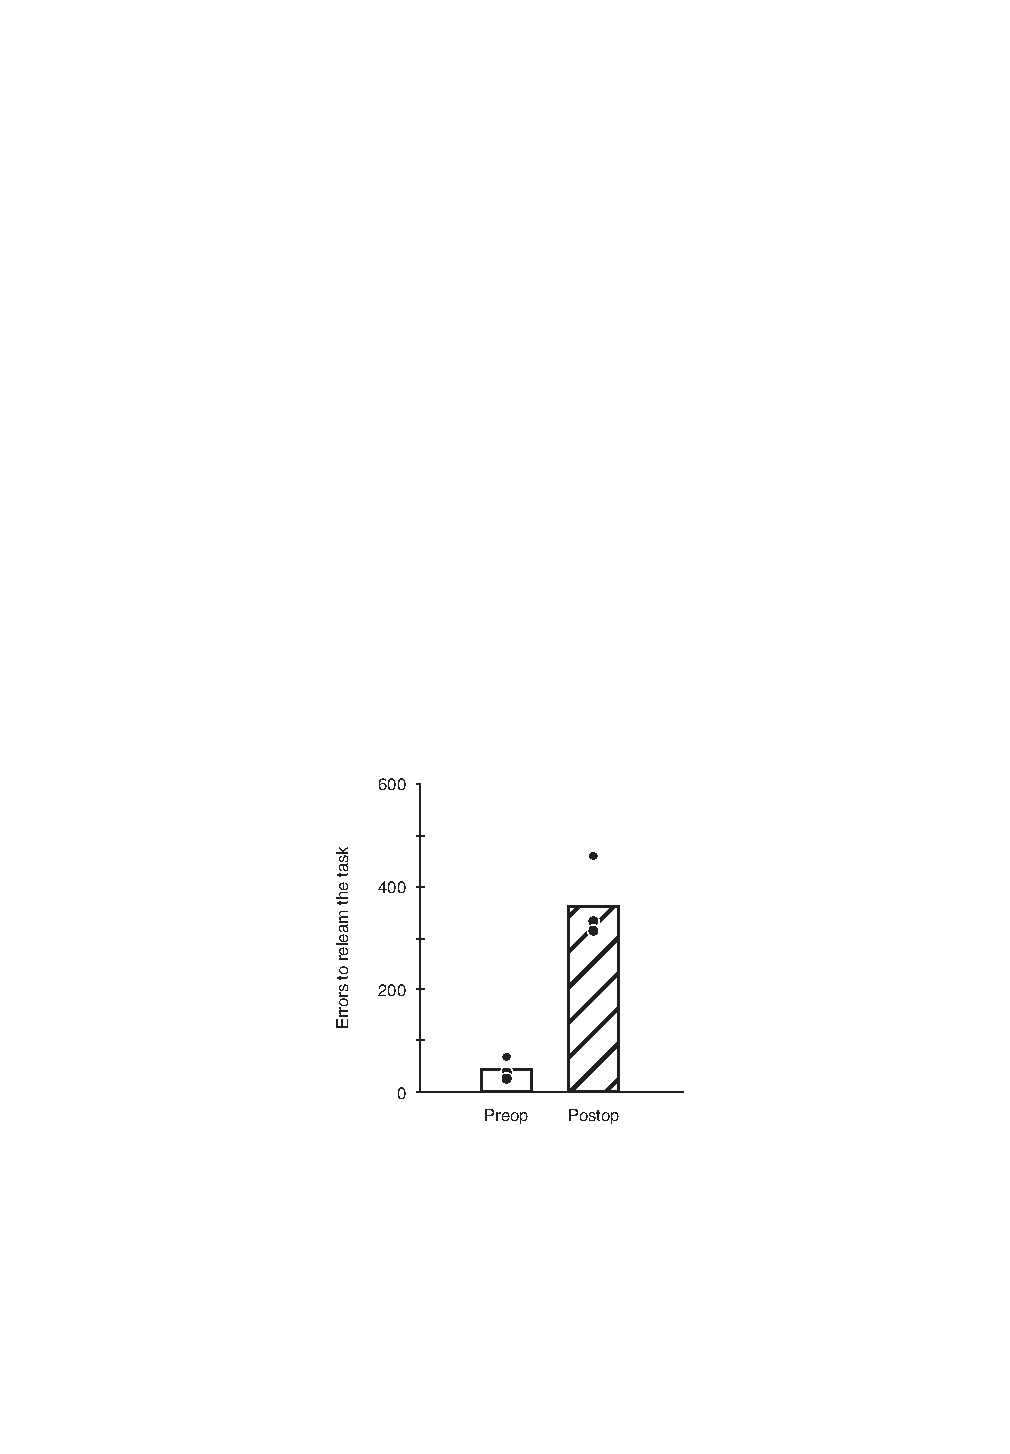
\includegraphics[width=0.45\linewidth]{chap7/7_3}
	\caption{腹侧前额叶皮层损伤对同步样本匹配任务的影响匹配。
		在同时匹配中,样本在选择时保持可见。
		一组猴子的\textit{术前}和\textit{术后}表现,在中断(白色条)和损伤后重新学习任务所需的错误数(阴影线)绘制在纵坐标上。
		实心圆圈表示个人的表现猴子\cite{rushworth1997ventral}。\label{fig:7_3}}
\end{figure}


\begin{figure}
	\centering
	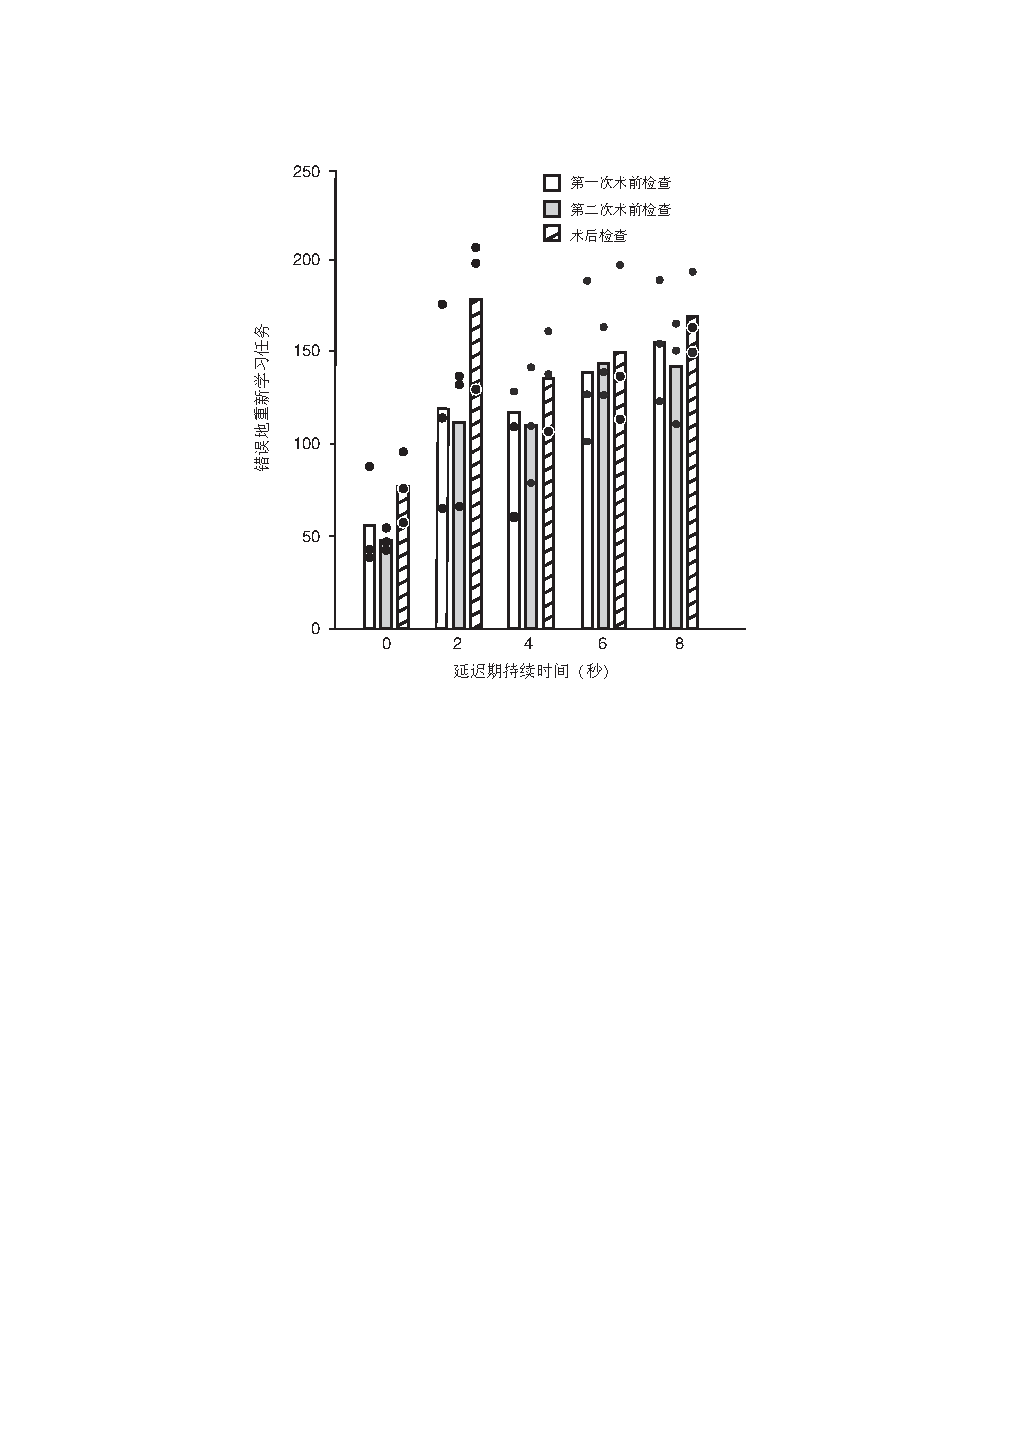
\includegraphics[width=0.64\linewidth]{chap7/7_4}
	\caption{腹侧前额叶皮层损伤对延迟匹配样本任务的影响,作为函数的延迟间隔。 
		两个术前测试的格式如图~\ref{fig:7_3}~所示(白色和灰色条)和损伤后的一项测试(阴影线)。
		腹侧前额叶皮层对工作记忆不是必需的\cite{rushworth1997ventral}。\label{fig:7_4}}
\end{figure}


\item 猴子可能会尝试记住样本,即使它们不需要,因此,结果可能反映了工作记忆的损害。
然而,这种解释无法解释 Rushworth 等人的研究结果。 
他们的猴子重新学习了同步匹配任务,因此 Rushworth 等人。
可以在样本和样本之间以不同的延迟时间重新测试受损的猴子选择刺激。 
与手术前相比,他们在延迟匹配方面没有犯更多错误(\ref{fig:7_4})。 
科瓦尔斯卡等\cite{kowalska1991role}同样发现,一旦有腹侧前额叶皮层的猴子病变重新学习了任务规则,它们在延迟的非匹配采样任务上正常执行,延迟时间长。
\par


我们知道延迟期活动发生在腹侧前额叶皮层和眶额皮层\cite{rosenkilde1981single,hoshi2000neuronal} 并且延迟期激活发生当人类受试者执行延迟匹配样本任务时\cite{rama2005functional,schon2008delayed}。
我们知道电刺激延迟期间的眶额皮层会导致猴子中这些任务的损伤\cite{sobotka2005can}。
所以我们不否认一些活动的存在用回顾性工作记忆来解释。 
而且我们不否认破坏这些区域的神经活动会导致这些任务的缺陷。 
然而,Rushworth 等人的结果。 
证明同时发生减值样本匹配任务不能归因于工作记忆问题:他们受伤的猴子在相当长的延迟后表现正常重新学习了任务规则。
\item 拒绝前两个说法留下了第三种可能的解释。 
损伤后,猴子不再知道任务规则,因此它们必须重新学习。 
在里面匹配样本任务,猴子必须使用身份规则:选择匹配样本的对象匹配样本。 
在本章的后面,我们引用了前额叶皮层中细胞活动的证据反映当前任务规则的皮层\cite{wallis2001single}。
造成的损害通过电刺激\cite{sobotka2005can}可能是由于未能保留规则。
\end{enumerate}



\subsection{总结}
\par 

本章至此,腹侧前额叶皮层在视觉或听觉线索到目标或行动的任意映射中起着关键作用。 
但是它的功能扩展了超越这样的协会。 
在匹配样本任务中,提示和目标不是任意的。 
当猴子在损伤前学习匹配规则时腹侧前额叶皮层,它们显示出在损伤后应用该规则的障碍。
然而,腹侧前额叶皮层损伤的猴子可以重新学习该规则,此后它们表现出正常的工作记忆能力。 
因此,它们对样本匹配任务的损害发生了,因为受损的猴子在受损后不再立即知道规则。



\section{分类}
\par

如果腹侧前额叶皮层有助于通过颜色或形状进行匹配,并且还有助于学习关联不同的图片,那么人们可能会期望它也会在学习刺激类别方面发挥作用。 
弗里德曼等人\cite{freedman2001categorical,freedman2002visual}使用延迟匹配样本任务教猴子区分猫和狗的图画。 
他们制作了一系列经过分级的变形图画,猴子学会了“猫”类别和“狗”类别之间的界限(图~\ref{fig:7_5})。
可以在延迟期间编码一个或另一个类别的腹侧前额叶皮层中找到细胞(图~\ref{fig:7_6})。


\begin{figure}
	\centering
	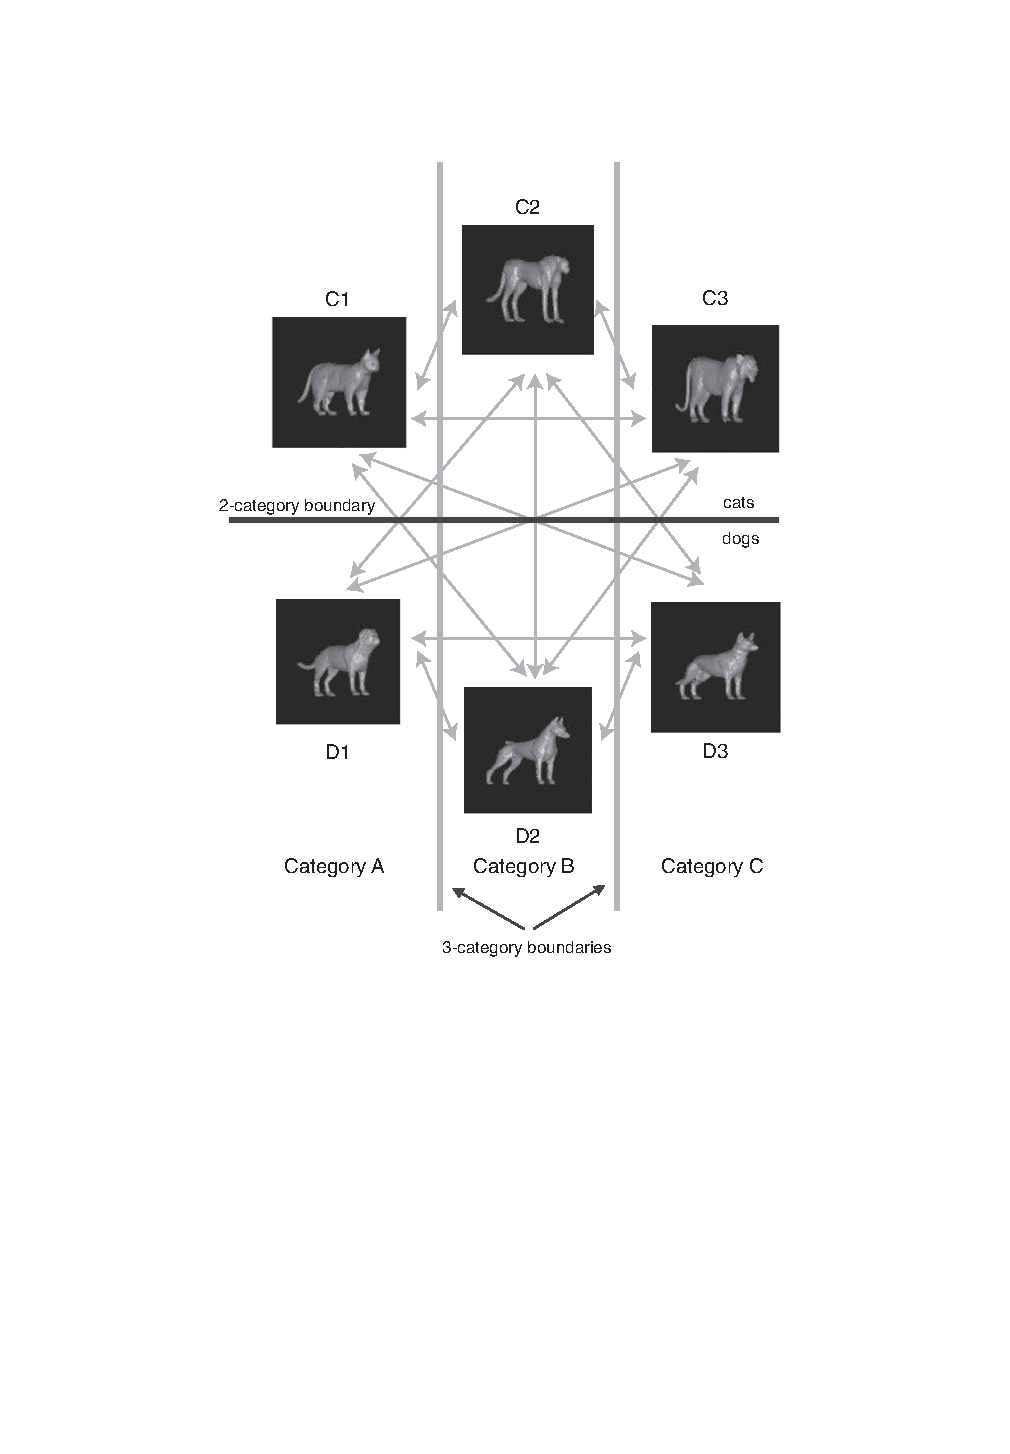
\includegraphics[width=0.6\linewidth]{chap7/7_5}
	\caption{分类任务中使用的刺激。
		实验者构建了由不同比例的箭头连接的 2 种刺激组成的图像。 
		3 只猫特辑 [C1 . . . C3] 和 3 只狗 [D1 . . . D3] 和它们的变形组合可以归类为狗与猫,由黑色水平线分隔。
		或者,可以根据 2 条灰色垂直线划定的 3 个类别,对相同的变形刺激进行任意分类\cite{freedman2002visual}。 \label{fig:7_5}}
\end{figure}
\par


研究人员继续教猴子新的类别。 
这涉及建立新的类别边界,如图~\ref{fig:7_4}~中的灰色垂直线所示。 
然后腹侧前额叶皮层中的细胞编码一个或另一个新类别(图~\ref{fig:7_7})。 
这一发现的重要性在于腹侧前额叶皮层可以学习的类别的任意性;
它们并不完全取决于共享功能的数量。
\par


扩展这些研究,Cromer 等人\cite{cromer2010representation}教会了猴子两个独立的类别:猫与狗以及跑车与轿车。
在这种情况下,他们发现了编码这两个类别的多任务细胞。 
但是当罗伊等人\cite{roy2010prefrontal}教猴子在猫狗分类的竞争方式之间切换,主要是独立的子种群对这些相互排斥的类别进行编码。 
这一结果类似于第~\ref{chap:chap6}~章提到的结果,其中背侧前额叶皮层中大部分独立的细胞亚群编码当前与先前的空间目标,这也是相互排斥的类别\cite{genovesio2006representation}。
\par


当然,这些发现并未表明腹侧前额叶皮层细胞对学习至关重要。 
下颞皮层可以学习类别,而前额叶皮层可以从那里检索信息。 
所以弗里德曼等人\cite{freedman2003comparison}研究了这 2 个领域的细胞。 
下颞叶皮层中的细胞确实编码了一些关于类别的信息,但是,与前额叶皮层中的细胞相比,它们的活动更多地反映了刺激的视觉特征(另见 Meyers\cite{meyers2008dynamic})。 
这一发现表明,下颞皮层比类别更能代表视觉特征和特征连词,并且分类学习发生在腹侧前额叶皮层。
\par

下颞皮层中代表特征结合的细胞(表示为 AB)自动编码具有这两种特征的对象类别,如图~\ref{fig:7_3}~所示。
因此,例如,仅具有 AB 特征的原型对象将被归类为具有附加特征的对象,例如 ABC、ABCD 等。
同样的原则适用于前额叶皮层内的分类。
\par


因此,类别编码和联合特征编码有着密切的关系,前额叶皮层和下颞皮层的区别不可能像类别和特征编码的区别那么简单。 
它们的不同之处在于,前额叶皮层从高阶和中阶连词中学习抽象,而下颞皮层仅学习中阶连词并且不太灵活。
例如,腹侧前额叶皮层似乎在学习具有特征 ABCD 和ABCE 可以属于类别 AB。 
但是它的细胞也可以了解到相同的 2 个对象属于类别 AC。 
下颞皮层学习中级连接 AB 和 AC 的灵活性似乎较低,主要基于特征而不是分类的附加因素。
\par


鉴于前额叶皮层和下颞皮层中的细胞活动都对类别进行编码,我们可能期望在人类受试者对图片进行分类时发现这 2 个区域的激活。 
DeGutis\cite{degutis2009network}教人们根据眼睛的高度和鼻子的长度将面孔分为 2 类。 
在学习这些类别的过程中,中外侧前额叶皮层和腹侧前额叶皮层的激活超过了练习类别,并且颞下回的激活仅在主题练习了一个类别。


\begin{figure}
	\centering
	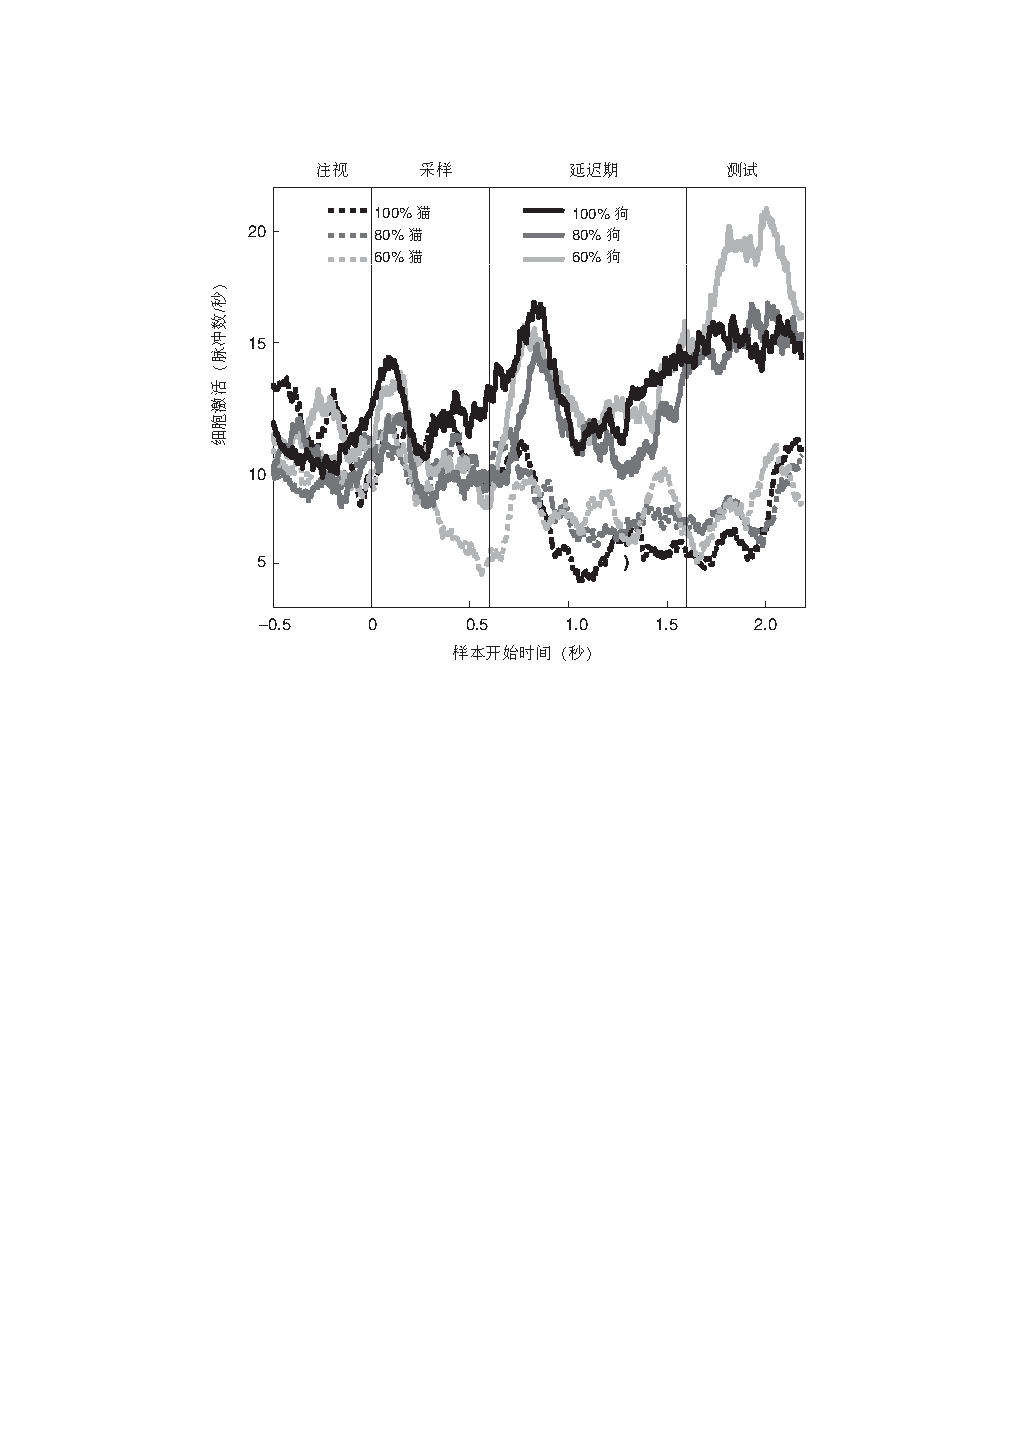
\includegraphics[width=0.62\linewidth]{chap7/7_6}
	\caption{编码“狗”类别的腹侧前额叶皮层细胞。
		实线显示细胞在试验中的活动,样本刺激完全(100\%)或主要(60\% 或 80\%)狗画。
		虚线表示完全或主要由猫画组成的试验活动。
		在延迟期和选择期(测试)期间,与“猫”类别相比,细胞对“狗”类别中的样本具有更高的活性\cite{freedman2002visual}。\label{fig:7_6}}
\end{figure}
\par


这些结果可以解释为什么当受试者将图片命名或归类为动物或工具时,激活通常不会发生在前额叶皮层中\cite{martin2007representation}。
相反,对于多种视觉类别,激活发生在颞叶,对于工具,激活发生在前运动皮层,大概是因为工具可以被处理。
前额叶皮层无法显示可检测的激活,因为受试者在早期教育中已经了解了动物和工具的类别。
对于成年人来说,将特定图片分配给一个或另一个类别是自动发生的。


\begin{figure}
	\centering
	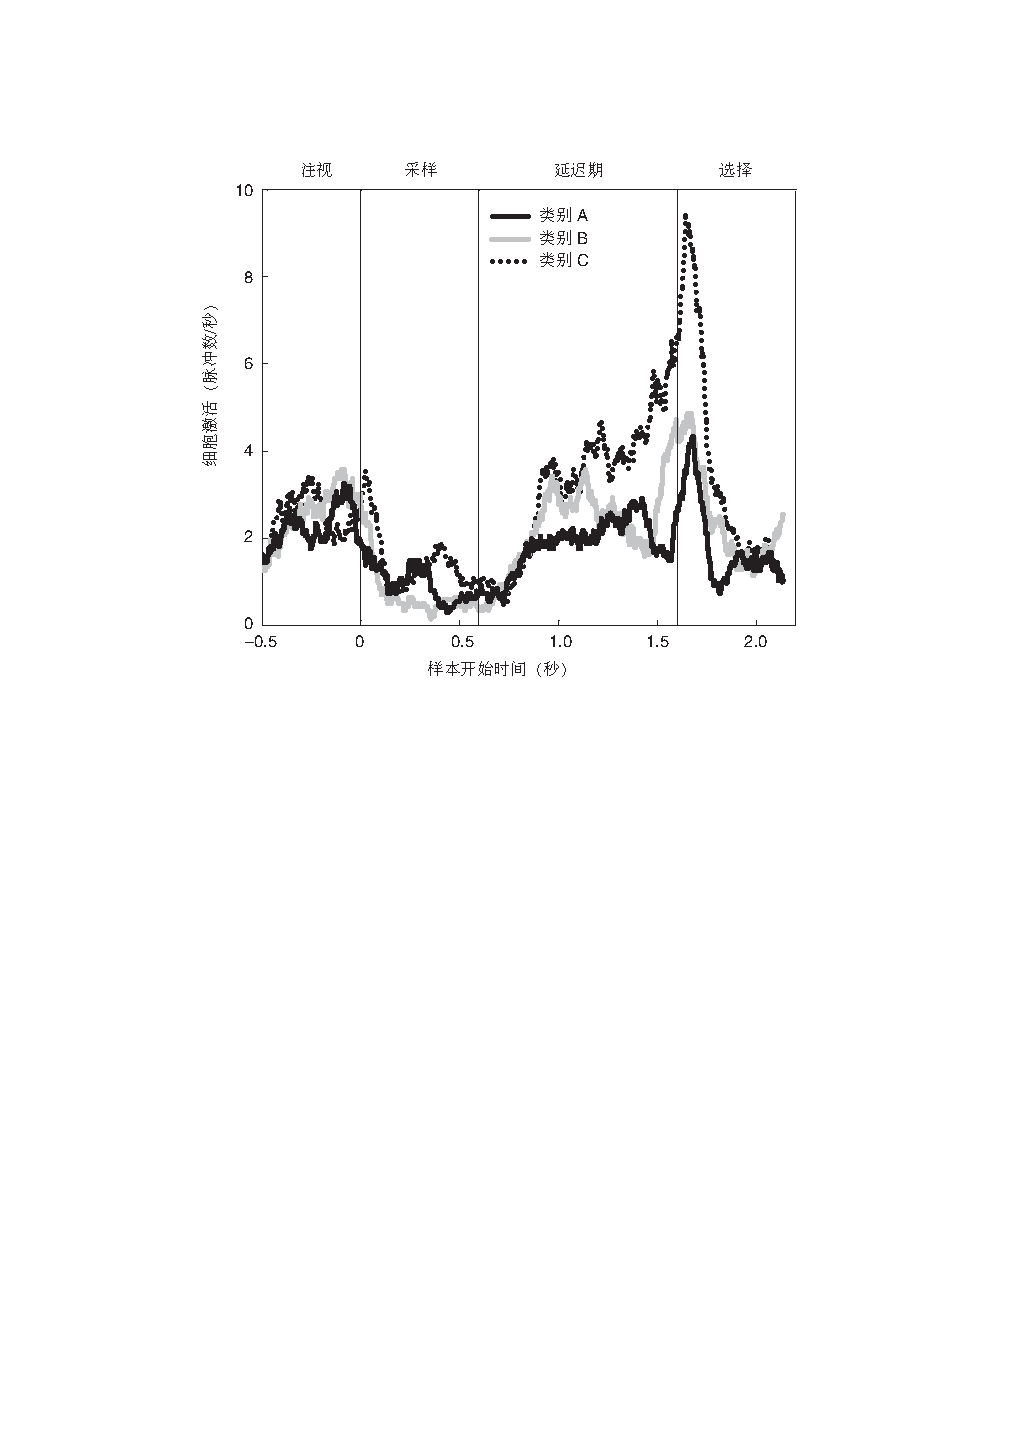
\includegraphics[width=0.62\linewidth]{chap7/7_7}
	\caption{编码任意类别的腹侧前额叶皮层细胞,由图~\ref{fig:7_5}~中的垂直灰线划分。
		该细胞偏好落在最右侧灰色垂直边界右侧的变形刺激,C 类\cite{freedman2002visual}。\label{fig:7_7}}
\end{figure}
\par


当然,我们并不是说成年人缺乏学习新概念和新范畴的能力。 
一个人可以教一只老狗新把戏。 
我们将在第~\ref{chap:chap8}~章讨论注意力与自动行为的相关主题。
就目前的目的而言,可以说对于训练良好的类别,相关的认知操作相对自动地发生,尤其是在成人中。
\par


当图片不属于一个简单的类别时,受试者必须设计新的类别。 
在这种情况下,前额叶皮层开始参与。 
因此,Degutis\cite{degutis2007distinct}发现,当他们将容易分类的面孔激活与更难分类的面孔激活进行比较时,激活仅针对困难的分类任务发生在中外侧前额叶皮层和腹侧前额叶皮层中。


\begin{figure}
	\centering
	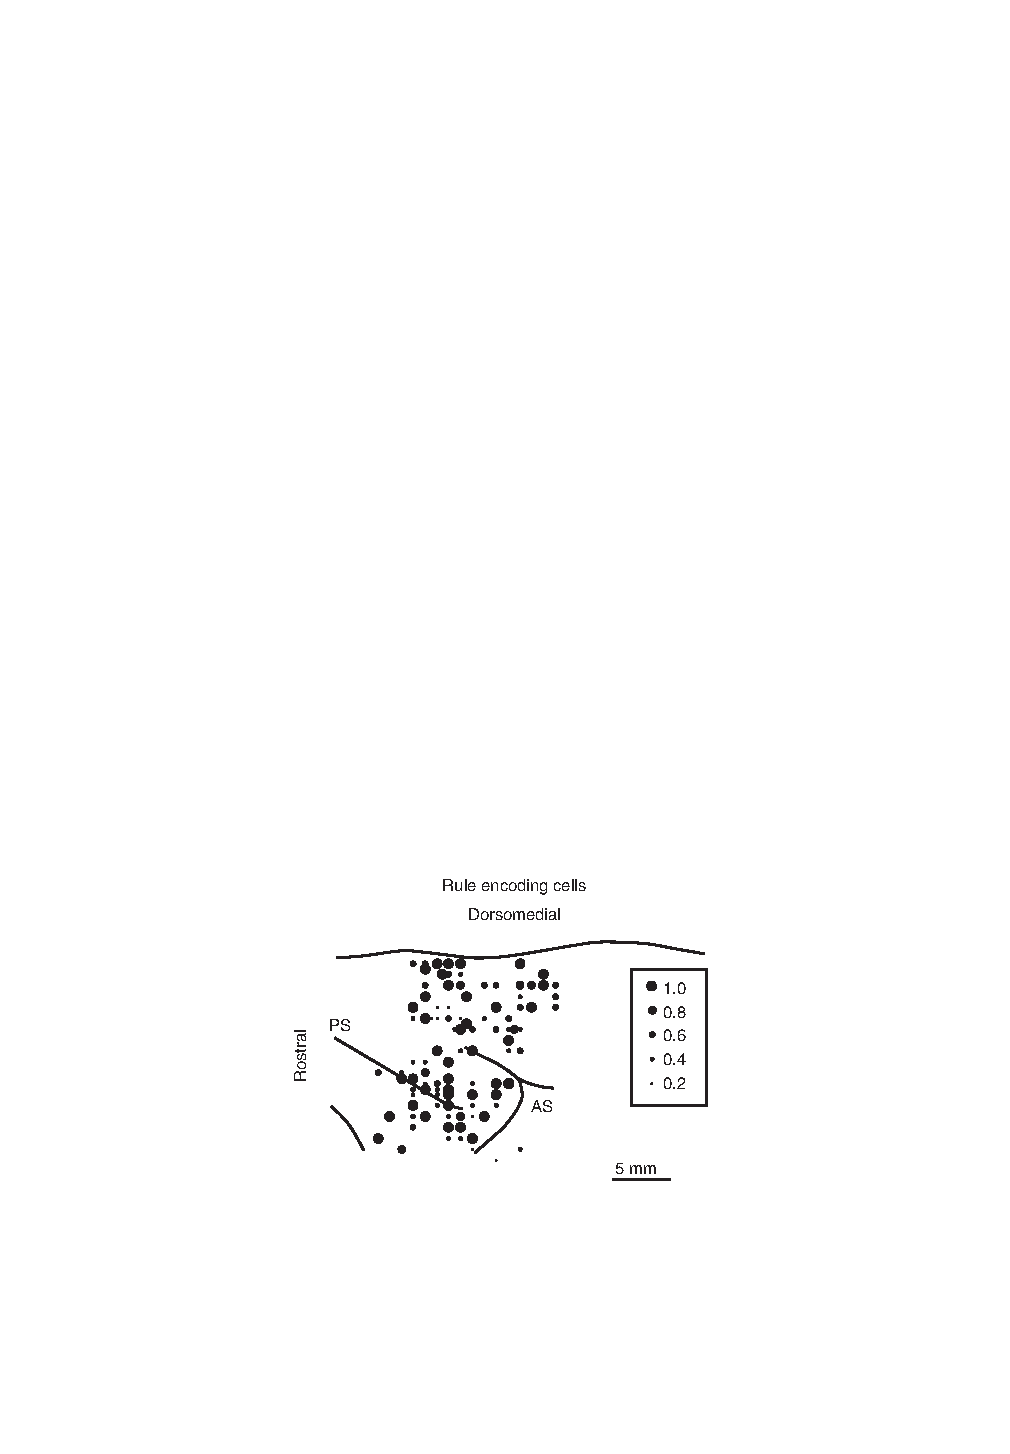
\includegraphics[width=0.6\linewidth]{chap7/7_8}
	\caption{规则编码细胞的位置。
		每个圆圈的直径显示在每个位点记录的编码两个规则之一的细胞的比例。
		一条规则要求使用颜色和形状刺激来选择目标; 另一个需要使用提示的位置来选择目标\cite{white1999rule}。 \label{fig:7_8}}
\end{figure}
\par


我们认为前额叶皮层通过从中阶和高阶联合表示中抽象来学习这些类别。 
我们还认为腹侧前额叶皮层可以做到这一点,而下颞叶皮层不能灵活地做到这一点。
和克罗默等人\cite{cromer2011comparison}表明前运动皮层中的细胞缺乏关于类别的信息,尽管那里的一些细胞活动反映了目标选择。 
因此,在不否认其他区域对分类和抽象的贡献的情况下,腹侧前额叶皮层似乎在这些功能中起着关键作用。
\par


然而,Mimaminoto 等\cite{monti2010willful}试图证明前额叶皮层甚至对于学习新类别也不是必需的。
他们训练猴子执行一项任务,其中刺激 A 预测一个级别的奖励,而刺激 B 预测另一个级别。 
用一点经验,猴子学会归纳;
也就是说,他们将具有刺激 A 某些特征的刺激视为刺激 A。
背侧前额叶皮层和腹侧前额叶皮层的联合损伤并没有阻止这种泛化。
\par


但是 Mimaminoto 等人使用的任务。
不需要猴子比较项目并在刺激之间构建任意划分,就像弗里德曼等人的实验那样。
Mimaminoto 等人的实验不是学习划分类别的任意细分,而是一种表征真正分类的属性。 
仅涉及刺激泛化,也称为特征泛化\cite{buckley2010top}。 
在刺激泛化中,如果动物已经知道刺激可以预测某事,那么当它看到一个共享其某些特征的刺激时,它也会预测同样的事情:
共享的特征越多,预测越强。
这种原始的知觉现象发生在所有脊椎动物身上,与分类无关。
\par


相比之下,弗里德曼等人使用的实验范式\cite{freedman2002visual}确实涉及分类。 
他们的猴子学会了根据任意划分将变形分为几类,而不是简单地根据一些共享特征。
例如,当他们看到狗的变体时,他们已经学会属于“狗”类别,他们稍后可以学习将相同的变体分类为“猫”。
关键区别涉及对象的学习和任意细分,如 Freedman 等人的实验,而不是 Mimaminoto 等人的实验中的自动刺激泛化。
因此,我们接受基于细胞记录的结论,这表明腹侧前额叶 皮层介导了基于学习的视觉对象的灵活分类。
\par


当猴子学会根据它们所属的类别选择对象时,前额叶皮层中的细胞活动会对该类别进行编码。
当猴子学习将刺激分类和重新分类到实验者选择施加的任何子集时,细胞会对这些类别进行编码。
尽管有包括腹侧前额叶皮层在内的病变的猴子仍然可以将刺激识别为相似,但它们是通过刺激泛化来识别的,这是一种系统发育上所有脊椎动物共有的古老机制,与真正的分类不同。
当猴子必须通过将任务规则应用于刺激类别(例如身份或匹配规则)来选择目标时,腹侧前额叶皮层发挥最大作用。



\subsection{总结}
\par
当猴子学会根据它们所属的类别选择对象时,前额叶皮层中的细胞活动会对该类别进行编码。
当猴子学习将刺激分类和重新分类到实验者选择施加的任何子集时,细胞会对这些类别进行编码。
尽管有包括腹侧前额叶皮层在内的病变的猴子仍然可以将刺激识别为相似,但它们是通过刺激泛化来识别的,这是一种系统发育上所有脊椎动物共有的古老机制,与真正的分类不同。
当猴子必须通过将任务规则应用于刺激类别(例如身份或匹配规则)来选择目标时,腹侧前额叶皮层发挥最大作用。



\section{抽象规则}
\par
弗里德曼等人的研究\cite{freedman2002visual}利用样本匹配规则来研究分类。 
这条规则是抽象的,因为它几乎可以应用于任何刺激。
\par


其他抽象规则具有相同的属性。
White\cite{white1999rule}发现尾侧、腹侧、后外侧和背侧前额叶皮层的活动编码了指导行为的规则。 
(\ref{fig:7_8})显示了记录站点。 
White 和 Wise 教猴子一个有条件的视觉运动规则和一个视觉空间规则,中央注视点的颜色指定了一组试验的规则。


\begin{figure}
	\centering
	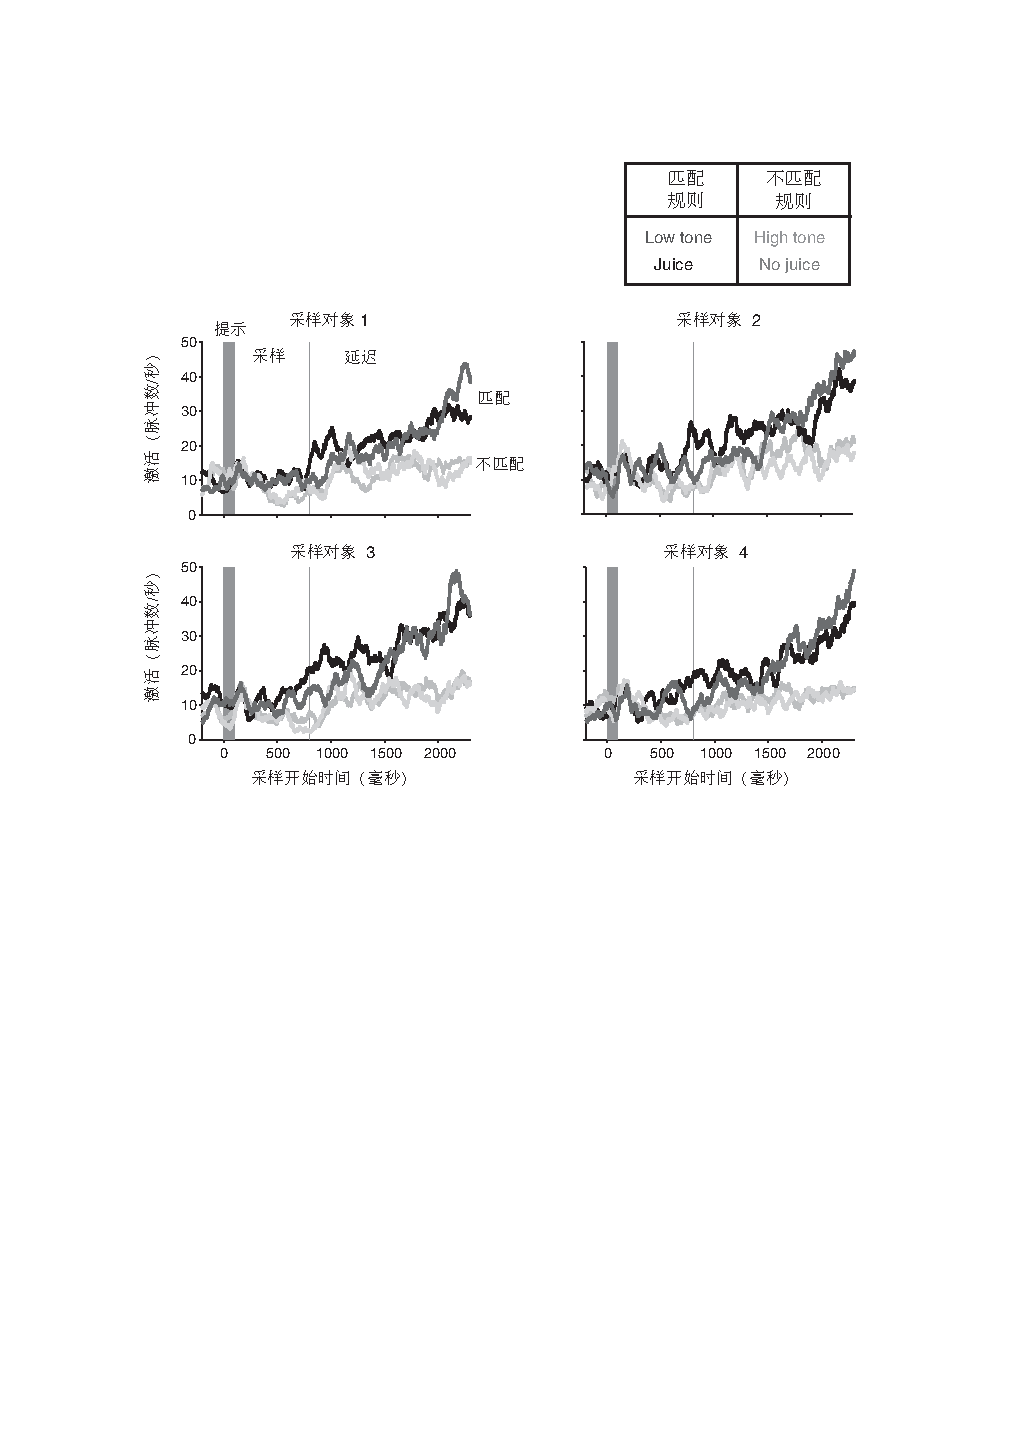
\includegraphics[width=0.7\linewidth]{chap7/7_9}
	\caption{匹配样本和非匹配样本任务中的规则编码单元。
		四种不同样本刺激的腹侧前额叶皮层细胞的活动 [对象 1。 . . 对象 4]。
		右上角的插图解释了指示猴子遵循以下两个规则之一的四个提示:匹配或不匹配。
		两个提示,低音调和果汁奖励的交付,指示匹配规则;
		两个不同的提示,高音调和在预期时间没有果汁输送,指示了不匹配规则。 
		暗线:匹配规则的单元格活动; 浅色线条:不匹配规则的活动\cite{wallis2001single}。 \label{fig:7_9}}
\end{figure}
\par


对于条件视觉运动规则,提示的形状和颜色告诉猴子选择哪个目标(在四个或八个可能的目标中),而对于空间规则,提示的位置就是如此。 
为了获得奖励,猴子需要对指示的目标进行扫视,然后在该位置的光点变暗时按下一个条。
\par


Hoshi等\cite{hoshi1998task}进行了类似的研究,但进行了伸手动作。 
他们从腹侧前额叶皮层的细胞中记录,而猴子则根据刺激形状(圆形和三角形)或位置选择到达目标。
许多细胞 (36\%) 根据两种形状对到达进行编码,偏好到达圆形或到达三角形(特征-目标连词)。
这些和其他细胞中的许多细胞(总共 34\%)根据规则对到达进行编码,优先选择基于刺激位置到达或基于形状到达。 
这些细胞编码规则与目标的结合,而不是运动本身。
\par


正如我们之前提到的,Wallis 等人\cite{wallis2001single}教猴子两条抽象规则:延迟匹配样本和延迟非匹配样本。 
然后他们在每次录音开始时呈现新奇的刺激。 抽象规则的应用不依赖于在任何给定试验中使用的项目的反复试验经验。 
当然,反复试验的经验在学习规则的过程中起着关键作用,但在这个实验中,猴子在记录细胞活动之前就已经很好地学习了规则。 
在 Wallis 等人的实验中,每次试验都会出现一张样本图片和一个提示,告诉猴子当前应用的规则是匹配还是不匹配。
\par


为了确保提示呈现后记录的任何细胞活动都反映了规则而不是提示的感官特性,Wallis 等人。
使用了两种截然不同的提示。
低音调或汁液输送指示猴子应用匹配规则,而高音调或没有汁液输送指示不匹配规则。
在每次试验中,这些说明之一与样本图片同时出现,在延迟期之前。 
通常,果汁被视为一种奖励,从技术上讲,人们可以在这些实验中这样看待它。
然而,在 Wallis 等人设计的任务中,果汁的输送(或不输送)为当前的试验提供了提示,就像指示相同规则的听觉信号一样。
\par


在样本和选择刺激之间的延迟期间,中外侧和腹侧前额叶 皮层中的一些细胞编码了匹配规则(\ref{fig:7_9}),而其他细胞编码了非匹配规则。 
这个结果既不依赖于刺激项目,也不依赖于指示规则的提示的性质\cite{wallis2001single}。
\par


在随后的研究中,穆罕默德等人\cite{muhammad2006comparison}当猴子执行同样的任务时,从下颞叶皮层记录下来。 
他们发现只有少数细胞编码规则。
这个结果可能反映了这样一个事实,即腹侧前额叶皮层,而不是下颞叶皮层,可以整合提示上下文、猴子选择的规则以及选择该规则的结果。
与腹侧前额叶皮层相比,下颞叶皮层对结果的直接和具体信息要少得多,腹侧前额叶皮层与眶额皮层有广泛的相互联系(第~\ref{chap:chap4}~章)。



\subsection{总结}
\par
前额叶皮层中的活动反映了当前的任务规则,例如,猴子是否应该选择与样本匹配的目标或不匹配的目标。
此活动发生在延迟期间,在规则指令呈现之后。
这些规则适用于任何刺激,无论是新奇的还是熟悉的,因此代表



\section{改变规则}
\par
抽象规则可以建立认知操作,例如匹配或不匹配,或者它可以指定与执行任务相关的刺激特征。 
Milner\cite{milner1963effects}为人类受试者改编了一项任务,以专门测试根据刺激特征改变规则的能力:威斯康星卡片分类任务。 
受试者根据每张卡片上的颜色形状将一系列卡片分成四堆。
\par


在任何一次试验中,受试者都可以根据卡片上设计的颜色、形状或数量对卡片进行分类。 
在标准版本的任务中,受试者在每次试验后都会收到反馈,但仅限于他们的选择是否正确。 
首先,受试者必须学会根据给定的特征(例如颜色)对卡片进行分类。 
实验者随后更改相关特征,例如,形状。 
主体仅从反馈中了解规则的变化,并通过一系列规则变化依次类推。
\par


大额叶切除术的患者犯了 MilnerMilner\cite{milner1963effects}所说的持续性错误,这种解释对文献产生了深远的影响——但我们认为是误导性的。 
这意味着患者在从先前成功的规则如何转换方面仍然存在一些特殊地问题。 
然而,这些患者不仅在改变现行规则方面存在障碍,而且在学习新规则和遵守规则方面也存在障碍。 
例如,Barcelo\cite{barcelo2002both}发现额叶大损伤患者会犯他们所谓的随机错误,以及顽固性错误。
\par


随机错误涉及在正确选择后犯错误:未能坚持最近成功的规则。 
(第~\ref{chap:chap4}~章)解释了在物体反转任务中,眶额皮层损伤的猴子也会在这个意义上犯随机错误\cite{rudebeck2008frontal}。
\par


这些错误反映了未能坚持基于积极反馈的正确选择。 (第~\ref{chap:chap3}~章)显示了内侧前额叶皮层的相同类型的结果。 
正如我们稍后解释的那样,当猴子学习条件性视觉运动任务时,腹侧前额叶皮层和眶额皮层病变会导致
“转移”和“留下”策略的相同损害\cite{bussey2001role}。
\par


因此,虽然我们承认额叶损伤会导致威斯康星卡片分类任务受损,但我们拒绝认为这种缺陷反映了行为抑制的失败或它是由坚持不懈造成的。 
(第~\ref{chap:chap4}~章)讨论了得出这个结论的一些原因,(第~\ref{chap:chap10}~章)再次更详细地讨论了这个主题。 
曼苏里等人\cite{mansouri2006prefrontal}为猴子设计了威斯康星卡片分类任务的简化版本。 
这些动物学会了根据颜色或形状来匹配刺激,只有奖励或非奖励作为反馈。 
(第~\ref{chap:chap3}~章)、(第~\ref{chap:chap4}~章) 和 (第~\ref{chap:chap6}~章)提到了这项任务的结果,分别针对内侧、眶额皮层和中外侧前额叶皮层的病变\cite{buckley2009dissociable}。
研究人员还损伤了腹侧前额叶皮层,但猴子在手术后未能重新学习任何匹配规则。
他们设法达到了大约 60\% 的正确率,但没有更好。
这一发现增加了腹侧前额叶皮层对抽象规则的学习和实施至关重要的证据。
\par


进一步的证据来自 Nakahara 等人的研究\cite{nakahara2002functional},他们在猴子和人身上使用成像方法,因为它们通过颜色或形状匹配,并且在这些规则之间转换。 
当受试者在规则之间转换时,激活位于猴子和人类腹侧前额叶皮层的尾部。 
人类的激活峰值接近 Monchi 等人报告的峰值\cite{monchi2001wisconsin}作为受试者收到威斯康星卡片分类任务的负面反馈。
Monchi等人专门分析了开关试验的数据,发现腹侧前额叶皮层(12/47 区)的峰值激活。
\par


Wisconsin 卡片分类任务有很多变量,因此 Hampshire\cite{hampshire2006fractionating}使用了不同的设计来更纯粹地衡量改变规则的能力。 
他们的实验比较了超维转移和维内转移。 
受试者首先学会区分两种复杂的刺激,如图~\ref{fig:7_10}~所示。
例如,受试者学会根据形状做出选择,同时忽略前景线条。
\par


然后受试者学习维度内转变,这要求他们区分两种新的复合刺激,相关刺激维度保持不变:在我们的例子中,形状而不是前景线。 
后来,受试者学习了一种超维度转变,这要求他们区分两种不同的新复合刺激,但另一个维度是相关的:在我们的例子中,前景线 Baxter\cite{baxter2007orbital}表明形状是内维度转变的显着特征,这意味着受试者不需要改变规则,而在超维度转变中他们确实需要从一个规则切换到另一个规则。


  \begin{figure}
  	\centering
  	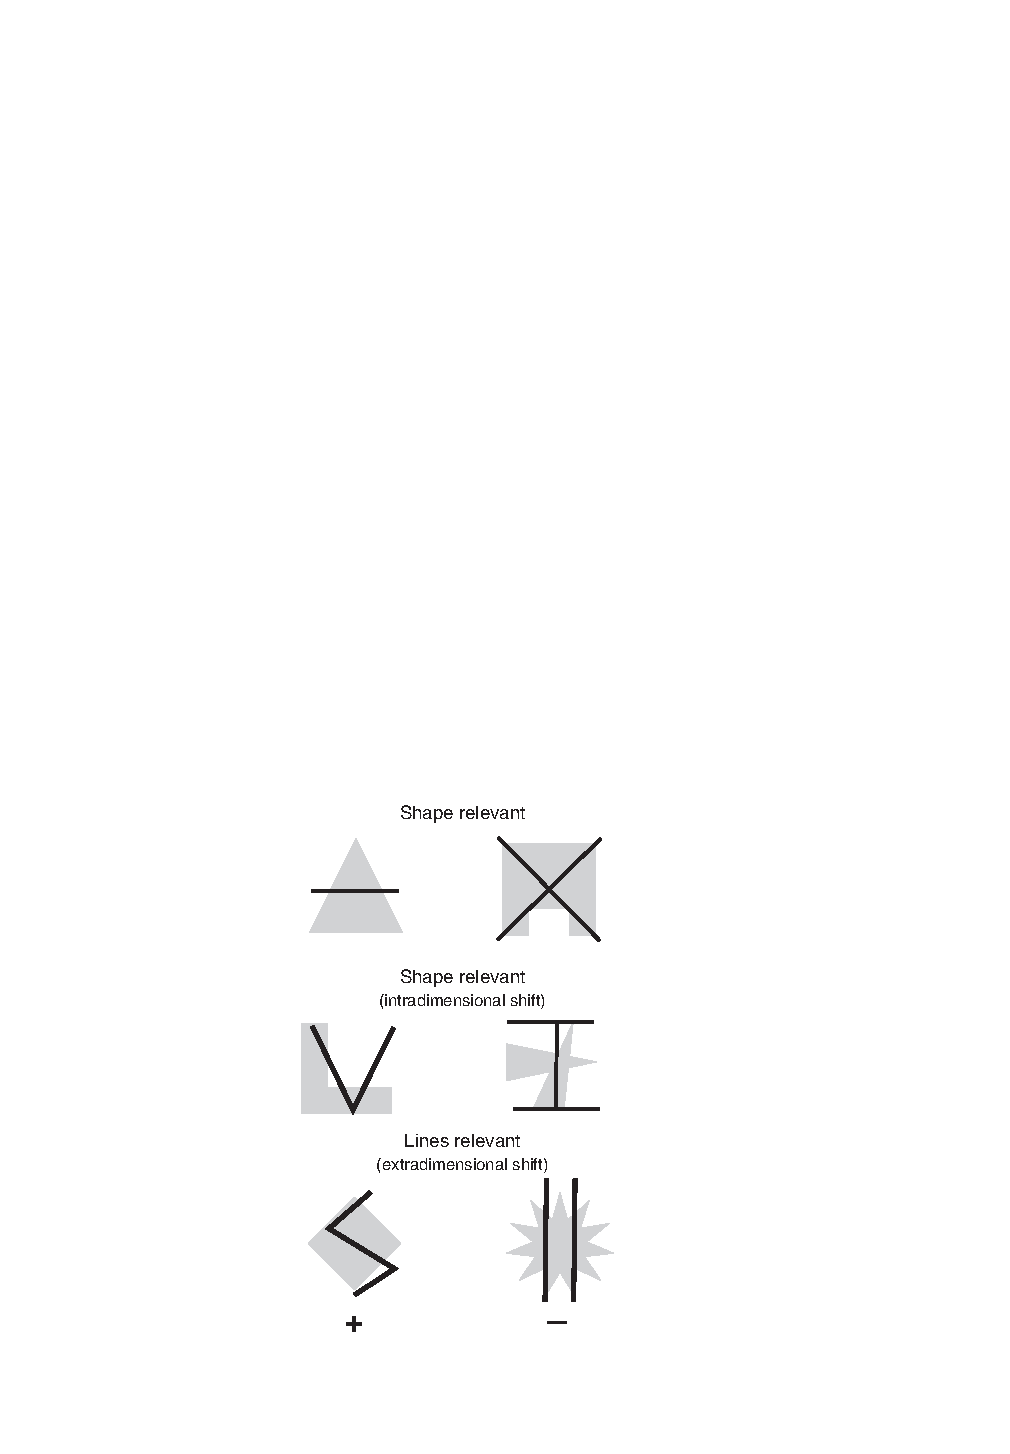
\includegraphics[width=0.6\linewidth]{chap7/7_10}
  	\caption{超维和内维转换任务的示例刺激。 
  		每对水平排列的复合刺激物代表一个选择。 
  		正确的、有奖励的选择在底部用 + 标记,不正确的选择用 — 标记\cite{dias1996primate}。\label{fig:7_10}}
  \end{figure}
\par


Hampshire\cite{hampshire2006fractionating}对比了维度外和维度内转移的激活,发现腹侧前额叶皮层的尾部对于涉及规则转移的任务(即维度外转移任务)有更大的激活。 
如前所述,峰值发生在 Monchi 等人附近\cite{monchi2001wisconsin}报告威斯康星卡片分类任务。
\par


正如人们所预料的那样,额叶切除术的患者比正常受试者在维度外移动上犯了更多错误,但在维度内移动上没有损伤\cite{owen1993contrasting}。
\par


迄今为止,还没有人通过这些任务对猕猴进行选择性损伤,但 Dias 等人。
\cite{dias1997dissociable}在普通的狨猴 (Callithrix) 中这样做了。 
他们比较了腹侧前额叶皮层凸面和眶额皮层损伤的影响。 
皮质皮质连接的模式表明前一个区域与猕猴的腹侧前额叶皮层(区域 12/47 和 45)同源\cite{roberts2007forebrain}。
\par


腹侧前额叶皮层凸面受损的狨猴可以学习超维位移,但与正常狨猴相比速度较慢\cite{dias1997dissociable}。
然而,他们在维度内转移时表现正常。 
这一发现进一步支持了腹侧前额叶皮层在指导行为的抽象规则中的作用。



\subsection{总结}
\par

腹侧前额叶皮层病变的猴子无法重新学习抽象规则,例如,通过颜色或形状进行匹配。
他们在改变规则方面也表现不佳,例如,在超维度轮班任务和威斯康星卡片分类任务中。



\section{抽象策略}
\par 
前面的部分提到了抽象规则。
我们所说的规则是指指定问题解决方案的输入-输出算法。
我们将这些与猴子在尝试解决问题时可以使用的策略区分开来(定义见词汇表)。
规则说明一个人必须做什么,而策略说明一个人可以做什么来解决问题。
\par 


为了说明我们所说的策略的含义,请考虑前面描述的条件视觉运动任务。 
如前所述,Bussey 等人\cite{bussey2001role}训练猴子解决一系列有条件的视觉运动问题。
每个彩色形状映射到三个或四个空间目标中的一个,并且只有一个。
实验者对新试验开始时做出的第一个选择进行评分,但也会在出现错误后使用更正程序,直到猴子做对为止。


 \begin{figure}
	\centering
	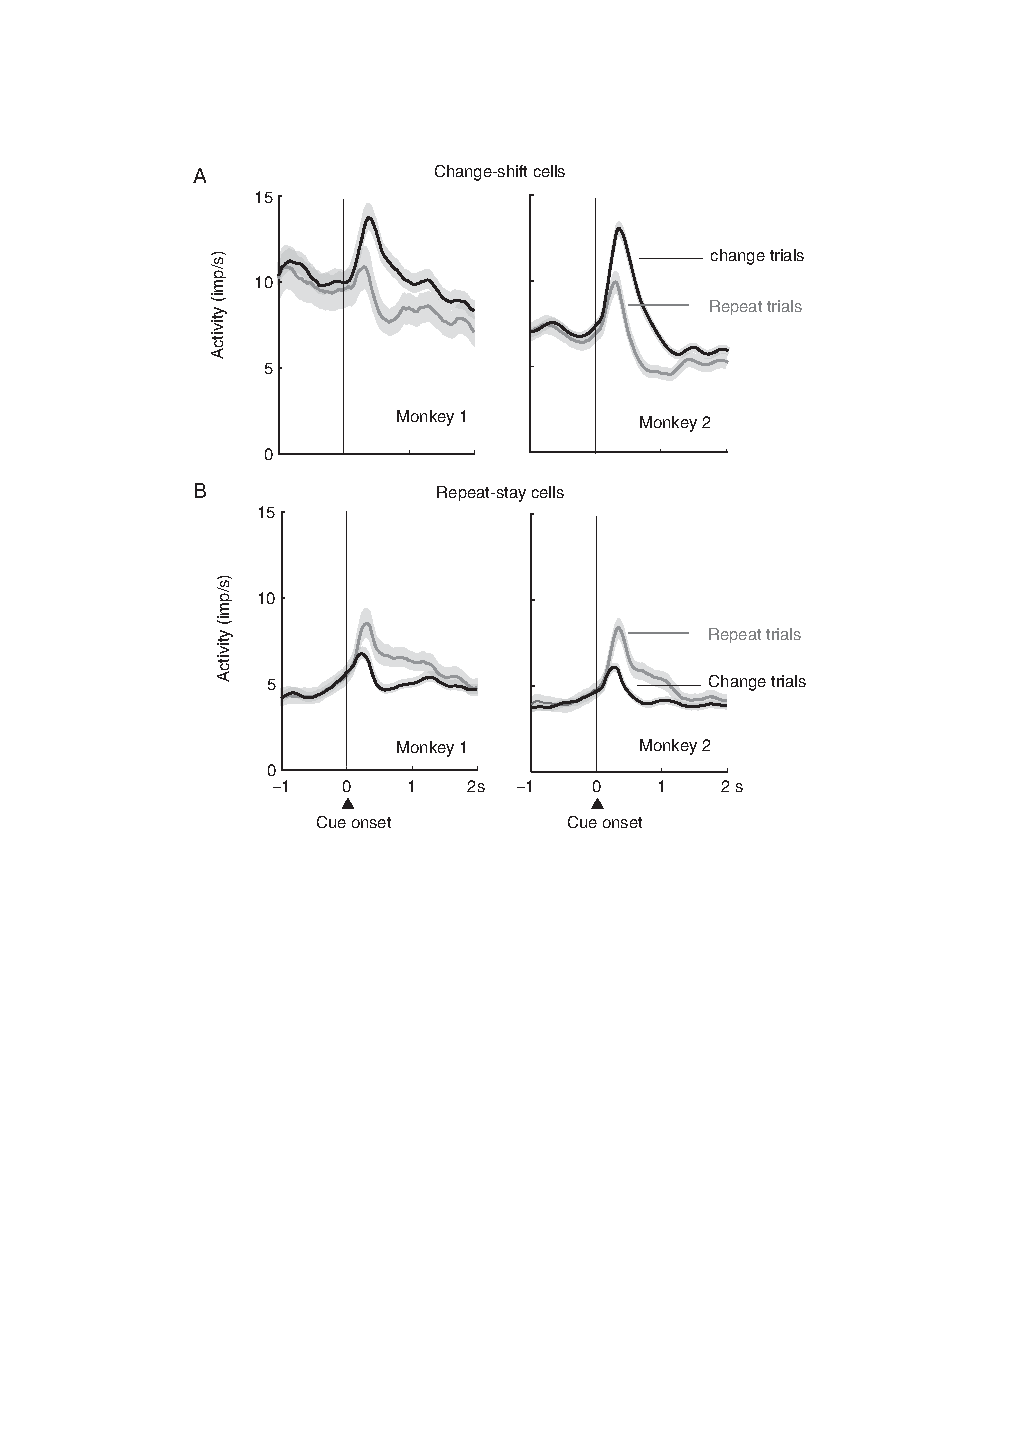
\includegraphics[width=0.6\linewidth]{chap7/7_11}
	\caption{抽象策略的人口编码。
		 (A) 编码两只猴子(左和右)变化转移策略的细胞的平均种群活动。
		 黑线:变化试验中的活动,在这些试验中,先前试验的提示发生变化表明猴子应该选择不同的目标。
		 灰线:重复试验的活动,这些试验具有与之前试验相同的提示。
		 阴影:SEM。
		 (B) 编码重复停留策略的细胞的群体活动。
		 格式如 (A) 所示\cite{genovesio2007neurophysiology}。\label{fig:7_11}}
\end{figure}
\par


在手术之前,但在解决此类问题的丰富经验之后,猴子很快就能学会新的提示-目标映射。
但他们也学到了其他东西。 他们学习了三种抽象策略:“重复-停留”、“变化-转移”和“失去-转移”。
根据第一种策略,如果提示从上一次试验中重复出现,猴子应该“停留”在同一个目标上。
根据第二种策略,如果线索与之前的试验不同,猴子应该“转移”到另一个目标。
根据第三种策略,如果猴子犯了错误,它应该“转移”到不同的目标。
\par


患有腹侧前额叶皮层和眶额皮层病变的猴子在手术后失去了应用所有这些策略的能力\cite{bussey2001role}。
我们在第~\ref{chap:chap8}~章(\ref{fig:8_6})中提供了关于这一点的更多证据。
在这里,我们再次诉诸第~\ref{chap:chap3}~章介绍的累加器-跑道模型来考虑策略实施的机制。 
累加器网络可以实施“变化-转移”策略,例如,通过整合该策略的“证据”。
当它达到阈值时,该网络可能会偏向目标网络的活动,从而使先前的目标无法“赢得”“比赛”。
这样一来,一个三选题就变成了一个二选题,错误率会因此下降约 17\%。
\par


吉诺维西奥等\cite{genovesio2005prefrontal}记录在猴子的前额叶皮层中,这些猴子被训练遵循“重复-停留”和“变化-转移”策略。
他们发现背侧前额叶皮层中的许多细胞,包括中外侧前额叶皮层,编码“重复停留”或“变化转移”策略(\ref{fig:7_11})。
策略编码并不简单地反映提示的变化或重复,因为一些细胞专门编码根据刺激选择的空间目标。
而且,在错误试验期间,策略编码在背侧前额叶皮层中变得非常弱或完全不存在\cite{genovesio2008encoding}。
Tsujimoto 等人\cite{tsujimoto2011comparison}发现眶额皮层中的细胞也对这些策略进行编码,并且他们表明眶额皮层中的细胞在中外侧前额叶皮层中的细胞之前这样做(第~\ref{chap:chap4}~章)。
\par 


加凡等人 ( 2002 ) 设计了一项任务来专门评估猴子学习抽象策略的能力,该策略涉及保持目标和从目标转移。
在他们的策略任务中,猴子学会了连续四次在屏幕上选择一个类似物体的刺激,然后只选择一次另一个刺激。
因此,为了以最佳方式执行每个问题,猴子必须将一组刺激分类为持续性刺激,将另一组刺激分类为零星刺激,并为每一类目标选择适当的次数。 
巴克斯特等人\cite{baxter2009ventrolateral}表明腹侧前额叶皮层的损伤会导致重新学习此类策略任务的显着缺陷。 
眶额皮层\cite{baxter2007orbital}和中外侧前额叶皮层\cite{baxter2008dorsolateral}的损伤没有这种影响。



\subsection{总结}
\par 
包括腹侧前额叶皮层在内的损伤会阻止猴子使用它们在损伤前自发学习的策略,而且它们似乎不会在损伤后重新学习这些策略。
抽象策略帮助猴子在面对新问题时使用他们在解决类似问题方面学到的知识来减少错误,即使这些策略不能完全消除错误。



\section{结论}

\subsection{腹侧前额叶皮层如何发挥作用}
\par

本章解释了腹侧前额叶皮层的连接如何支持其独特的功能。


\begin{enumerate}
\item 腹侧前额叶皮层根据可见标志生成目标。 
连同感觉事件的顺序、时间和位置~\ref{chap:chap6},这些标志构成了当前行为环境的重要组成部分。
腹侧前额叶皮层可以执行其功能,因为它与下颞叶皮层和鼻周皮层相连,它们代表物体和其他视觉特征的结合。
\item 基于听觉信号的目标生成取决于它与上颞叶皮层的联系。
它可能对基于与顶叶区域连接的体感刺激具有类似的功能。
\item 腹侧前额叶皮层还通过其与眶额皮层的连接接收有关结果的信息,以及直接来自与杏仁核的连接以及通过眶额皮层间接接收的当前需求信息。
因此,根据当前的生物学需求评估,它可以为当前环境和期望的结果生成适当的目标。
\item 它与运动前区的联系可能解释了它在条件视觉运动映射中的作用,尽管精确的路径仍然不确定;
与下颞叶皮层的连接介导条件性视觉-视觉关联。
\item 腹侧前额叶皮层分别通过与颞叶皮层、前额叶和运动前区以及眶额皮层的连接接收有关背景、目标和输出的会聚输入。
在下一章中,我们提出了这样一种观点,即前额叶皮层位于处理上下文、目标和结果的层次结构的顶端。
由于其在这些层次结构中的地位,腹侧前额叶皮层不仅可以生成具体目标,还可以生成抽象目标,例如目标集、类或类别; 应避免的地方和物体; 以及具体和抽象目标的各种组合。
例如,“换班”策略通过避免地点或行动产生一组潜在目标。
\item 腹侧前额叶皮层不仅可以产生抽象目标,还可以产生基于抽象规则和策略的目标。 
指示规则和策略的信号可能取决于与用于音调的\textit{上颞皮层}\cite{wallis2001single}、用于颜色的\textit{下颞皮层}\cite{tsujimoto2010evaluating}以及眶额皮层皮层、杏仁核的连接 , 或多巴胺能神经元的结果。
抽象的规则和策略允许猴子将他们在类似情况下学到的知识应用到新的刺激中。
\item 腹侧前额叶皮层介导的认知操作也可以增强其他皮层区域的表征。
第~\ref{chap:chap5}~章解释了腹侧前额叶皮层通过自上而下的注意影响皮层感觉区域的信息处理。
腹侧前额叶皮层与下颞和鼻周皮层的连接使其既能调节视觉规则和策略,又能使感觉处理偏向相关刺激。
它与尾侧前额叶皮层的连接也有助于发挥这一作用。
因此,如果任务规则涉及形状或颜色,则腹侧前额叶皮层与下颞皮层的连接(直接和间接通过尾侧前额叶皮层)使其能够影响相关区域的表征。
\end{enumerate}




\subsection{提议}
\par

这些想法引导我们提出以下建议,首先是简要形式,然后进行了一些扩展。
\begin{enumerate}
\item 简单来说:
根据当前需求评估,腹侧前额叶皮层生成适合当前环境和期望结果的目标。 
目标可以是对象、位置或动作,可以是具体的也可以是抽象的。
\item  展开来说:
腹侧前额叶皮层根据构成当前环境的视觉和听觉信号生成目标。
目标的产生还取决于根据当前需求评估的预期结果。 
除了物体和地点等具体目标外,腹侧前额叶皮层还会生成抽象目标,例如要选择或避免的一组、类别或类别的目标。 
它还根据抽象规则和策略生成目标。 通过与尾侧前额叶皮层和感觉区域的互连,它将接收到的信息偏向与当前任务相关的特征。
\end{enumerate}



\subsection{为什么其他皮层区域不能做腹侧前额叶皮层做的事情}
\par

我们提出腹侧前额叶皮层可以执行这些功能,而其他大脑区域不能,我们这样做的原因很简单:它的连接。
例如,在有条件的视觉运动任务中,猴子必须学会将提示和动作与结果联系起来。
我们之前解释了腹侧前额叶皮层如何获得建立这些连接所需的信息:分别来自时间、运动前和眼眶皮层的提示、动作和结果。
大脑皮层的其他部分无法直接获得所有这些信息。
一些区域,例如后顶叶皮层,与杏仁核或眶额皮层缺乏牢固的联系。
一些,例如上颞皮层和下颞皮层,缺乏进入腹侧前额叶皮层所具有的运动前区的那种途径。
而其他的,例如运动前皮层,不接收来自颞叶皮层的输入,而腹侧前额叶皮层则接收到这些输入。
\par


批评者可能反对其中一些结论。
例如,后顶叶皮层具有到运动前区的视觉输入和输出。
事实上,细胞可以记录在后顶叶区域 LIP 中,该区域对提示的颜色或其空间位置是否指定适当动作的方向进行编码\cite{toth2002dynamic}。
也有报道称后顶叶皮层中存在编码形状的细胞\cite{janssen2008coding}; 所以背侧和腹侧视觉流之间的分离并不像有时描述的那样绝对。
此外,我们说后顶叶皮层没有从眶额皮层接收到太多输入,但这并不意味着它缺乏任何关于结果的信息。
例如,我们知道后顶叶皮层中的细胞编码奖赏的大小或概率\cite{platt1999neural},并且它们接收来自中脑多巴胺能神经元的输入。
对我们结论的批评者可能会对运动前皮层提出类似的论点。
\par


尽管有这些反对意见,我们坚持认为后顶叶皮层不会像腹侧 前额叶皮层和前运动皮层那样接收关于食物视觉和味道的详细信息。 
这两个区域都与代表特定结果的眶额皮层没有直接联系(第~\ref{chap:chap4}~章),并且前运动皮层和杏仁核之间只有稀疏的联系\cite{avendan1983evidence}。
正是由于这个原因,上顶叶皮层或下顶叶皮层的损伤对条件视觉运动任务的再学习没有影响\cite{rushworth1997parietal}。
\par 


至于前运动皮层,它当然会导致条件视觉运动任务受损\cite{halsband1985premotor,petrides2019conditional}。
但是,尽管腹侧前额叶皮层中的细胞编码视觉信号,但运动前皮层中的细胞主要编码即将到来的运动\cite{pllegrino1991neurophysiological}。
因此,腹侧前额叶皮层,而不是后顶叶或运动前皮层,能够根据视觉信号产生目标。



\subsection{对觅食选择的贡献}
\par

腹侧前额叶皮层在类人灵长类动物中随着大脑和身体的扩张而进化,这是在灵长类动物中央凹的进化以及三色视觉的发展之后发生的。
类人猿的单栖动物祖先采用了一种昼夜觅食策略,这种策略促进了在做出觅食选择时使用远距离线索。
在野外,视觉和听觉标志表明资源的可用性。
类人灵长类动物精致的全彩色视觉使它们能够辨别远处食物或其他资源的迹象,以及当地觅食地块中食物和液体的质量。
它们的腹侧前额叶皮层还允许类人猿将这种视觉信息与来自竞争对手和同类的声音相结合,这些声音也可以作为资源的标志。
例如,(第~\ref{chap:chap2}~章)解释说,类人猴的觅食选择似乎通常取决于它们在树上看到或听到的东西,而它们对附近地区的物品的选择在很大程度上取决于同一类型的区分食物视觉特性的细微变化。
\par


(第~\ref{chap:chap3}~章)到(第~\ref{chap:chap7}~章)逐个区域探讨前额叶皮层,因为它的连接因区域而异。
探索到此结束。
本书的其余部分将作为一个整体处理前额叶皮层。 
在下一章中,我们建议它具有简单的基本功能。

